% Figure 1 (variant): Linear taxonomy with ALIGN band — standalone file
% Drop into the paper with % Figure 1 (variant): Linear taxonomy with ALIGN band — standalone file
% Drop into the paper with % Figure 1 (variant): Linear taxonomy with ALIGN band — standalone file
% Drop into the paper with % Figure 1 (variant): Linear taxonomy with ALIGN band — standalone file
% Drop into the paper with \input{figure_linear}
%
% Requires: tikz, xcolor
% Compile:  pdflatex figure_linear.tex

\documentclass[tikz,11pt]{standalone}
\usepackage{xcolor}
\usepackage{tikz}
\usetikzlibrary{arrows.meta, positioning, calc, shadows}

\definecolor{okblue}{HTML}{0072B2}
\definecolor{okorange}{HTML}{E69F00}
\definecolor{okgreen}{HTML}{009E73}
\definecolor{okred}{HTML}{D55E00}
\definecolor{okyellow}{HTML}{F0E442}
\definecolor{okgray}{HTML}{999999}

\begin{document}
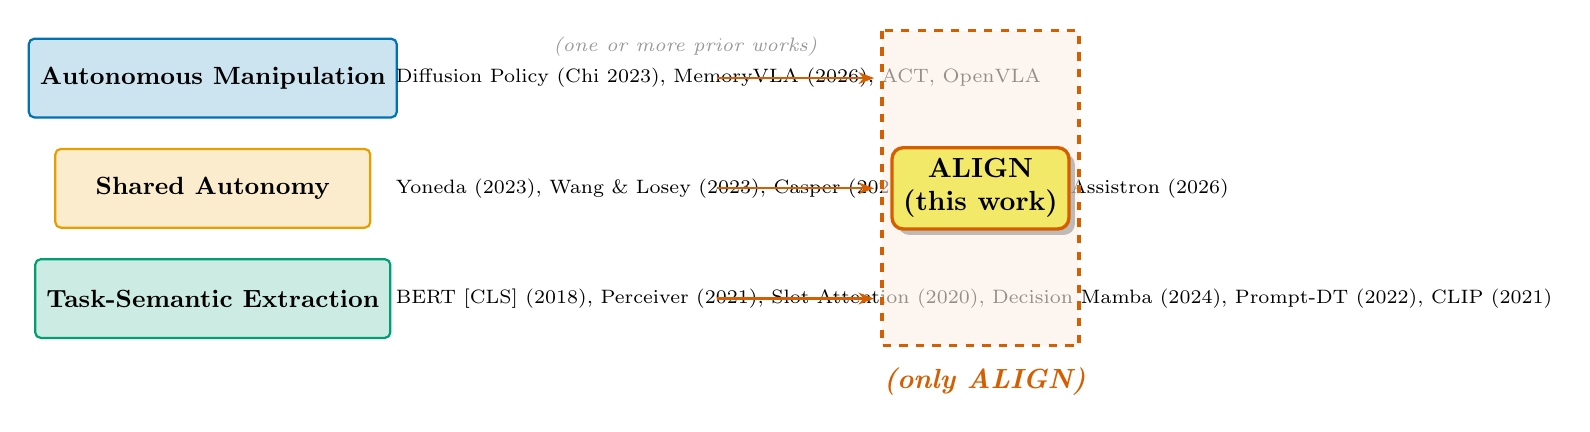
\begin{tikzpicture}[
    every node/.style={font=\small},
    row/.style={rectangle, rounded corners=2pt, draw, thick,
                minimum height=1.0cm, inner sep=4pt},
]
\node[row, fill=okblue!20, draw=okblue, minimum width=4cm]
    at (0, 0) {\bfseries Autonomous Manipulation};
\node[row, fill=okorange!20, draw=okorange, minimum width=4cm]
    at (0, -1.4) {\bfseries Shared Autonomy};
\node[row, fill=okgreen!20, draw=okgreen, minimum width=4cm]
    at (0, -2.8) {\bfseries Task-Semantic Extraction};

\node[align=left, font=\scriptsize, anchor=west] at (2.2, 0)
    {Diffusion Policy (Chi 2023), MemoryVLA (2026), ACT, OpenVLA};
\node[align=left, font=\scriptsize, anchor=west] at (2.2, -1.4)
    {Yoneda (2023), Wang \& Losey (2023), Casper (2025), RT-V3 (2026),
     Assistron (2026)};
\node[align=left, font=\scriptsize, anchor=west] at (2.2, -2.8)
    {BERT [CLS] (2018), Perceiver (2021), Slot Attention (2020),
     Decision Mamba (2024), Prompt-DT (2022), CLIP (2021)};

\draw[okred, very thick, dashed, fill=okred!10, fill opacity=0.6]
    (8.5, 0.6) rectangle (11, -3.4);
\node[draw=okred, very thick, fill=okyellow!80, rounded corners,
      align=center, font=\bfseries, drop shadow, inner sep=4pt]
    at (9.75, -1.4) {ALIGN\\(this work)};

\foreach \y in {0, -1.4, -2.8} {
    \draw[-{Stealth[length=2mm]}, okred, thick]
        (6.4, \y) -- (8.4, \y);
}

\node[font=\scriptsize\itshape, color=okgray, anchor=west]
    at (4.2, 0.4) {(one or more prior works)};
\node[font=\bfseries\itshape, color=okred, anchor=west]
    at (8.4, -3.85) {(only ALIGN)};

\end{tikzpicture}
\end{document}

%
% Requires: tikz, xcolor
% Compile:  pdflatex figure_linear.tex

\documentclass[tikz,11pt]{standalone}
\usepackage{xcolor}
\usepackage{tikz}
\usetikzlibrary{arrows.meta, positioning, calc, shadows}

\definecolor{okblue}{HTML}{0072B2}
\definecolor{okorange}{HTML}{E69F00}
\definecolor{okgreen}{HTML}{009E73}
\definecolor{okred}{HTML}{D55E00}
\definecolor{okyellow}{HTML}{F0E442}
\definecolor{okgray}{HTML}{999999}

\begin{document}
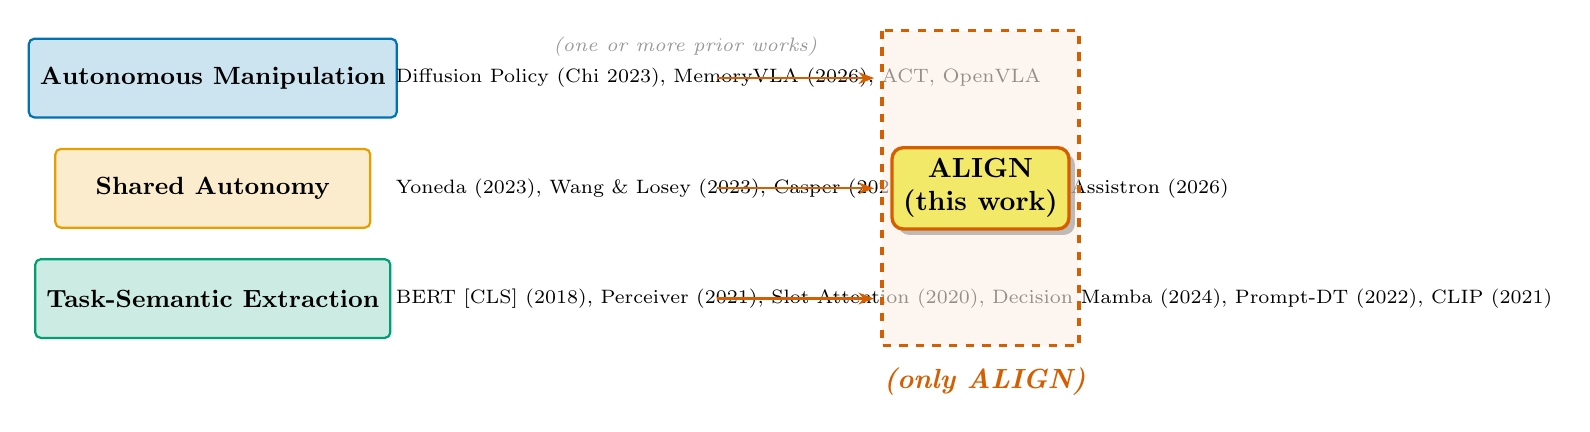
\begin{tikzpicture}[
    every node/.style={font=\small},
    row/.style={rectangle, rounded corners=2pt, draw, thick,
                minimum height=1.0cm, inner sep=4pt},
]
\node[row, fill=okblue!20, draw=okblue, minimum width=4cm]
    at (0, 0) {\bfseries Autonomous Manipulation};
\node[row, fill=okorange!20, draw=okorange, minimum width=4cm]
    at (0, -1.4) {\bfseries Shared Autonomy};
\node[row, fill=okgreen!20, draw=okgreen, minimum width=4cm]
    at (0, -2.8) {\bfseries Task-Semantic Extraction};

\node[align=left, font=\scriptsize, anchor=west] at (2.2, 0)
    {Diffusion Policy (Chi 2023), MemoryVLA (2026), ACT, OpenVLA};
\node[align=left, font=\scriptsize, anchor=west] at (2.2, -1.4)
    {Yoneda (2023), Wang \& Losey (2023), Casper (2025), RT-V3 (2026),
     Assistron (2026)};
\node[align=left, font=\scriptsize, anchor=west] at (2.2, -2.8)
    {BERT [CLS] (2018), Perceiver (2021), Slot Attention (2020),
     Decision Mamba (2024), Prompt-DT (2022), CLIP (2021)};

\draw[okred, very thick, dashed, fill=okred!10, fill opacity=0.6]
    (8.5, 0.6) rectangle (11, -3.4);
\node[draw=okred, very thick, fill=okyellow!80, rounded corners,
      align=center, font=\bfseries, drop shadow, inner sep=4pt]
    at (9.75, -1.4) {ALIGN\\(this work)};

\foreach \y in {0, -1.4, -2.8} {
    \draw[-{Stealth[length=2mm]}, okred, thick]
        (6.4, \y) -- (8.4, \y);
}

\node[font=\scriptsize\itshape, color=okgray, anchor=west]
    at (4.2, 0.4) {(one or more prior works)};
\node[font=\bfseries\itshape, color=okred, anchor=west]
    at (8.4, -3.85) {(only ALIGN)};

\end{tikzpicture}
\end{document}

%
% Requires: tikz, xcolor
% Compile:  pdflatex figure_linear.tex

\documentclass[tikz,11pt]{standalone}
\usepackage{xcolor}
\usepackage{tikz}
\usetikzlibrary{arrows.meta, positioning, calc, shadows}

\definecolor{okblue}{HTML}{0072B2}
\definecolor{okorange}{HTML}{E69F00}
\definecolor{okgreen}{HTML}{009E73}
\definecolor{okred}{HTML}{D55E00}
\definecolor{okyellow}{HTML}{F0E442}
\definecolor{okgray}{HTML}{999999}

\begin{document}
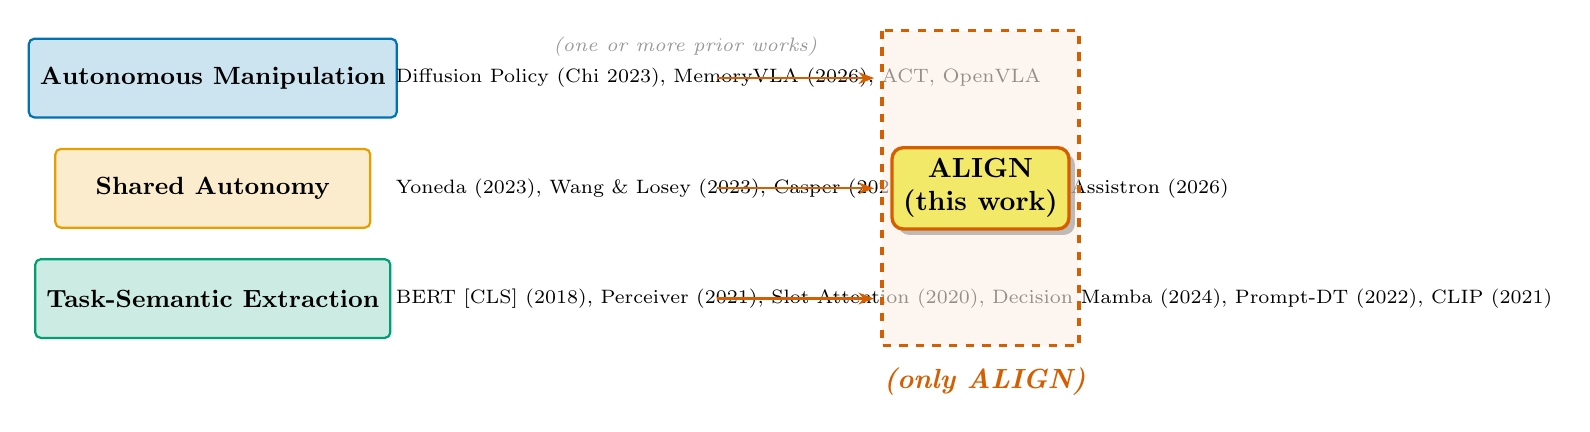
\begin{tikzpicture}[
    every node/.style={font=\small},
    row/.style={rectangle, rounded corners=2pt, draw, thick,
                minimum height=1.0cm, inner sep=4pt},
]
\node[row, fill=okblue!20, draw=okblue, minimum width=4cm]
    at (0, 0) {\bfseries Autonomous Manipulation};
\node[row, fill=okorange!20, draw=okorange, minimum width=4cm]
    at (0, -1.4) {\bfseries Shared Autonomy};
\node[row, fill=okgreen!20, draw=okgreen, minimum width=4cm]
    at (0, -2.8) {\bfseries Task-Semantic Extraction};

\node[align=left, font=\scriptsize, anchor=west] at (2.2, 0)
    {Diffusion Policy (Chi 2023), MemoryVLA (2026), ACT, OpenVLA};
\node[align=left, font=\scriptsize, anchor=west] at (2.2, -1.4)
    {Yoneda (2023), Wang \& Losey (2023), Casper (2025), RT-V3 (2026),
     Assistron (2026)};
\node[align=left, font=\scriptsize, anchor=west] at (2.2, -2.8)
    {BERT [CLS] (2018), Perceiver (2021), Slot Attention (2020),
     Decision Mamba (2024), Prompt-DT (2022), CLIP (2021)};

\draw[okred, very thick, dashed, fill=okred!10, fill opacity=0.6]
    (8.5, 0.6) rectangle (11, -3.4);
\node[draw=okred, very thick, fill=okyellow!80, rounded corners,
      align=center, font=\bfseries, drop shadow, inner sep=4pt]
    at (9.75, -1.4) {ALIGN\\(this work)};

\foreach \y in {0, -1.4, -2.8} {
    \draw[-{Stealth[length=2mm]}, okred, thick]
        (6.4, \y) -- (8.4, \y);
}

\node[font=\scriptsize\itshape, color=okgray, anchor=west]
    at (4.2, 0.4) {(one or more prior works)};
\node[font=\bfseries\itshape, color=okred, anchor=west]
    at (8.4, -3.85) {(only ALIGN)};

\end{tikzpicture}
\end{document}

%
% Requires: tikz, xcolor
% Compile:  pdflatex figure_linear.tex

\documentclass[tikz,11pt]{standalone}
\usepackage{xcolor}
\usepackage{tikz}
\usetikzlibrary{arrows.meta, positioning, calc, shadows}

\definecolor{okblue}{HTML}{0072B2}
\definecolor{okorange}{HTML}{E69F00}
\definecolor{okgreen}{HTML}{009E73}
\definecolor{okred}{HTML}{D55E00}
\definecolor{okyellow}{HTML}{F0E442}
\definecolor{okgray}{HTML}{999999}

\begin{document}
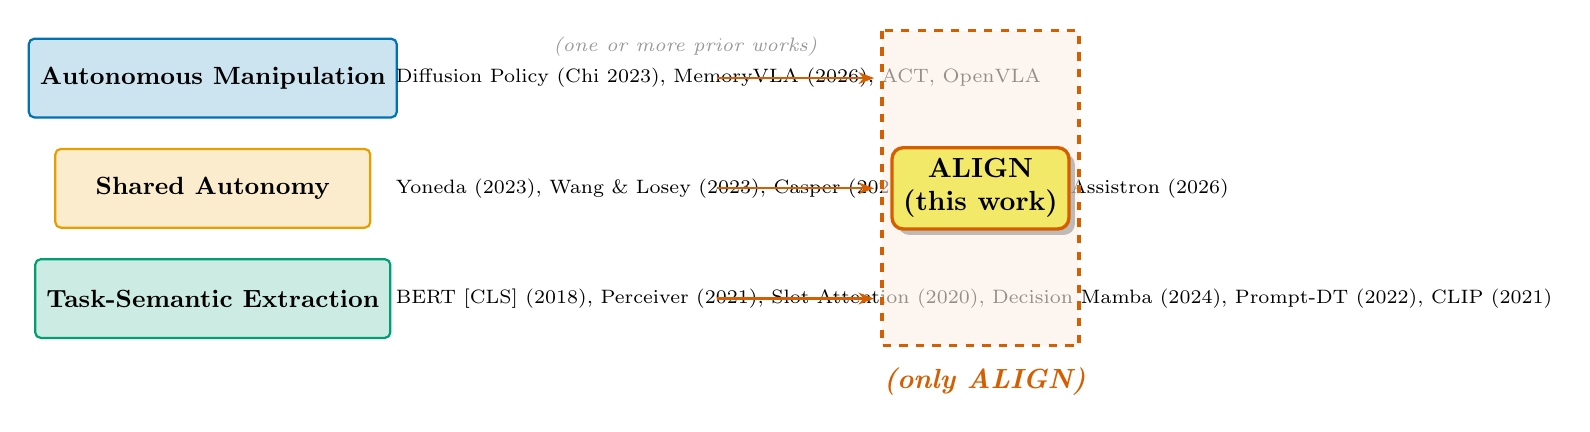
\begin{tikzpicture}[
    every node/.style={font=\small},
    row/.style={rectangle, rounded corners=2pt, draw, thick,
                minimum height=1.0cm, inner sep=4pt},
]
\node[row, fill=okblue!20, draw=okblue, minimum width=4cm]
    at (0, 0) {\bfseries Autonomous Manipulation};
\node[row, fill=okorange!20, draw=okorange, minimum width=4cm]
    at (0, -1.4) {\bfseries Shared Autonomy};
\node[row, fill=okgreen!20, draw=okgreen, minimum width=4cm]
    at (0, -2.8) {\bfseries Task-Semantic Extraction};

\node[align=left, font=\scriptsize, anchor=west] at (2.2, 0)
    {Diffusion Policy (Chi 2023), MemoryVLA (2026), ACT, OpenVLA};
\node[align=left, font=\scriptsize, anchor=west] at (2.2, -1.4)
    {Yoneda (2023), Wang \& Losey (2023), Casper (2025), RT-V3 (2026),
     Assistron (2026)};
\node[align=left, font=\scriptsize, anchor=west] at (2.2, -2.8)
    {BERT [CLS] (2018), Perceiver (2021), Slot Attention (2020),
     Decision Mamba (2024), Prompt-DT (2022), CLIP (2021)};

\draw[okred, very thick, dashed, fill=okred!10, fill opacity=0.6]
    (8.5, 0.6) rectangle (11, -3.4);
\node[draw=okred, very thick, fill=okyellow!80, rounded corners,
      align=center, font=\bfseries, drop shadow, inner sep=4pt]
    at (9.75, -1.4) {ALIGN\\(this work)};

\foreach \y in {0, -1.4, -2.8} {
    \draw[-{Stealth[length=2mm]}, okred, thick]
        (6.4, \y) -- (8.4, \y);
}

\node[font=\scriptsize\itshape, color=okgray, anchor=west]
    at (4.2, 0.4) {(one or more prior works)};
\node[font=\bfseries\itshape, color=okred, anchor=west]
    at (8.4, -3.85) {(only ALIGN)};

\end{tikzpicture}
\end{document}
